\documentclass{report}

\usepackage[]{indentfirst}
\renewcommand{\thesection}{\arabic{section}}
\usepackage{outlines}
\usepackage{booktabs}
\usepackage{graphicx}
\usepackage{nicematrix}
\usepackage{multicol}
\usepackage{circuitikz}
\usepackage[table,xcdraw]{xcolor}
\usepackage{amsmath,amsthm,amssymb}
\usepackage[export]{adjustbox}
\usepackage[backend=biber, style=numeric]{biblatex}

\graphicspath{{images}}
\addbibresource{EEE104.bib}
\newtheorem{theorem}{Theorem}
\newtheorem{lemma}{Lemma}
\renewcommand\qedsymbol{$\blacksquare$}
\ctikzset{logic ports=ieee}

\begin{document}
\title{\textbf{EEE104 Lab Report:}\\ Digital Electronics\\ \small (version 1)}
\author{Felix Lianto (2362727)}
\maketitle

\section{Introduction}
	Digital circuits have become the backbones for a lot of electronics we use today. They are frequently used to translate voltage values into logic levels, which the designer could use to implement computer logic and build a computer from the ground up. Implementations of these circuits can be found within small, rudimentary gadgets up to general purpose computers and smartphones. \\

	\underline{This laboratory report aims to:}
	\begin{enumerate}
		\item Understand Boolean Algebra and its corresponding theorems.
		\item Implement and observe basic logic gates individually and combinational logic circuits.
		\item Implement and observe basic types of memory circuits.
	\end{enumerate} 
	
	\subsection{Preliminary Information}
	The world works in analog systems, which means that their values can be measured and are always continuous \autocite{widmerDigitalSystemsPrinciples2018}. This can be observed and analyzed using the methods of continuous mathematics, such as calculus, and experimental observations. However, these systems are not the easiest to work with, given their nature that things cannot be precisely exact when working with continuous values. This is where digital systems can be useful for those specific circumstances.
	
	Digital systems only works under binary states, that is, only one of two possible values are allowed for any given digital system \autocite{widmerDigitalSystemsPrinciples2018}. For example, a switch is a digital system as it can only be turned on or turned off, nothing else. In digital systems, only a range of values are important to analyze, not a precise value. This fundamental principle behind digital systems is the backbone behind all smart devices built today.
	
	\subsubsection{Logic Circuits: Basic Logic Gates, Boolean Algebra, and DeMorgan's Theorem}
	To convert random binary states into something meaningful, it is important to understand the significance of logic gates. Logic gates can operate on one or more input signals and output another binary signal based on its rules. As an example, consider the NOT gate. The NOT gate considers only one input signal and outputs the inverse of that signal. This means that if an input of OFF is fed, it outputs ON, and vice-versa. Indeed, these gates can be compounded into more complicated circuitry, hence the need for an algebraization to simplify these logical circuits. \\
	
	This can be remedied by an algebraic structure known as Boolean Algebra. First introduced by George Boole in 1847 \autocite{booleLogicMathematicalAnalysis2015}, this system can formally transform a logical circuit into an algebraic expression, where the variables only have binary states. Table \ref{table:1} shows the algebraic representation of the gates, while Figure \ref{figure:1} highlights some basic theorems from such a system.
	
	\begin{table}[h]
		\centering
		\begin{NiceTabular}{@{}c|cc@{}}
			\toprule
			Logic Gate                & \begin{tabular}[c]{@{}c@{}}Diagram of\\ Logic Gate\end{tabular} & \begin{tabular}[c]{@{}c@{}}Equivalent Boolean \\ Expression\end{tabular} \\ \midrule
			Buffer                    							&\includegraphics[scale=0.5,valign=M]{buffer}                                     &$A$                                                                         \\
			NOT &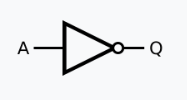
\includegraphics[scale=0.5,valign=M]{NOT}                                                                   
			&$\overline{A}$                                                                 \\
			\midrule AND &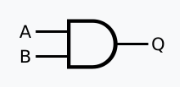
\includegraphics[scale=0.5,valign=M]{AND}                                                                   
			&$AB$                                                                       \\
			OR  &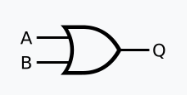
\includegraphics[scale=0.5,valign=M]{OR}                                                                   
			&$A+B$                                                                          \\
			\midrule NAND &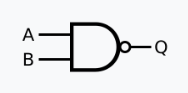
\includegraphics[scale=0.5,valign=M]{NAND}                                                                   
			&$\overline{AB}$                                                                \\
			NOR &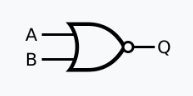
\includegraphics[scale=0.5,valign=M]{NOR}                                                                   
			&$\overline{A+B}$                                                                \\
			\midrule XOR &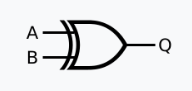
\includegraphics[scale=0.5,valign=M]{XOR}                                                                   
			&$\overline{A}B + A\overline{B}$                                                                \\
			XNOR &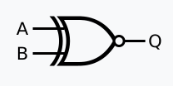
\includegraphics[scale=0.5,valign=M]{XNOR}                                                                   
			&$AB + \overline{A} \cdot \overline{B}$                                                                \\
			 \bottomrule
		\end{NiceTabular}
		\caption{Fundamental logic gates, its circuit diagram (according to the IEEE Standard Graphic Symbols for Logic Functions or IEEE/ANSI 91/91a-1984), and its equivalent boolean expression \autocite{LogicGate2024}.}
		\label{table:1}
	\end{table}
	
	\begin{figure}[h]
		\centering
		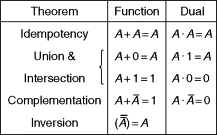
\includegraphics{booleanaxioms}
		\caption{Fundamental Theorems of Boolean Algebra \autocite{holdsworthBooleanAlgebra2002}}
		\label{figure:1}
	\end{figure}
	
	From these theorems, we can prove important theorems that can help with simplification of boolean expressions. One such theorem is the DeMorgan's Theorem, commonly used to separate joint variables under a NOT operator \autocite{widmerDigitalSystemsPrinciples2018};
	
	\begin{lemma}[Negation by Complementary Law \autocite{shinobiAnswerVerifyDemorgans2017}]
		\label{negByComplement}
		For any boolean variable $B$, $A = \overline{B}$ if and only if $AB = 0$ and $A + B = 1$.
	\end{lemma}
	
	\begin{proof}
		Suppose that $A = \overline{B}$. Clearly, by the complementary law, we have the desired result.
		
		Now suppose that $AB = 0$ and $A + B = 1$. Then, notice that
		\begin{align*}
			A + B &= 1 \\
			(A + B)\overline{B} &= 1 \cdot \overline{B} \\
			A\overline{B} + B\overline{B} &= \overline{B} \\
			A\overline{B} &= \overline{B}
		\end{align*}
		Then, since we know that $AB = 0$, we have,
		\begin{align*}
			AB &= 0 \\
			A\overline{B} + AB &= \overline{B} + 0 \\
			A(B + \overline{B}) &= \overline{B} \\
			A &= \overline{B}
		\end{align*}
		Thus, the lemma is proven \autocite{shinobiAnswerVerifyDemorgans2017}.
	\end{proof}
	
	\begin{lemma}[Absorption Law]
		\label{absorp}
		For any boolean variable $A$ and $B$, we have
		\begin{align*}
			A + AB &= A \\
			A + \overline{A}B &= A + B
		\end{align*}
	\end{lemma}
	
	\begin{proof}
		Notice that for the first statement,
		\begin{align*}
			A + AB &= A \cdot (1 + B) \\
			&= A
		\end{align*}
		and for the second statement,
		\begin{align*}
			A + \overline{A} &= (A + \overline{A})(A + B) \\
			&= 1 \cdot (A + B) \\
			&= A + B
		\end{align*}
		Thus, the claim holds.
	\end{proof}
	
	\begin{theorem}[DeMorgan's Theorem]
		For any boolean variable $A$ and $B$, we have
		\begin{align}
			\overline{AB} = \overline{A} + \overline{B} \label{deMorganNAND} \\
			\overline{A+B} = \overline{A} \cdot \overline{B} \label{deMorganNOR}
		\end{align}
	\end{theorem}
	
	\begin{proof} (Statement \ref{deMorganNAND}) 
		Notice, by Lemma \ref{negByComplement}, that it is sufficient to show that $AB + (\overline{A} + \overline{B}) = 1$ and $AB(\overline{A} + \overline{B}) = 0$ in order to prove statement \ref{deMorganNAND}. Observe that
		\begin{align*}
			AB + (\overline{A} + \overline{B}) &= \overline{B} + (AB + \overline{A}) &\text{(Rearrange)}\\
			&= \overline{B} + (\overline{A} + B) &\text{(Lemma \ref{absorp})} \\
			&= \overline{A} + (B + \overline{B}) &\text{(Rearrange, Identity)}\\
			&= \overline{A} + 1 = 1 &\text{(Complementation, Identity)}
		\end{align*}
		and also
		\begin{align*}
			AB(\overline{A} + \overline{B}) &= A\overline{A}B + AB\overline{B} &\text{(Distributivity)} \\
			&= 0 \cdot B + A \cdot 0 &\text{(Inverses)} \\
			&= 0 + 0 = 0 &\text{(Identity)}
		\end{align*}
		Therefore, the result follows.
	\end{proof}
	
	\begin{proof} (Statement 2)
		We can utilize the first statement to prove this second statement. Observe that
		\begin{align*}
			\overline{A+B} &= \overline{\overline{\overline{A}} + \overline{\overline{B}}} &\text{(Inversion)}\\
			&= \overline{\overline{\overline{A} \cdot \overline{B}}} &\text{(First statement)} \\
			&= \overline{A} \cdot \overline{B} &\text{(Inversion)}
		\end{align*}
		Thus, the result is proven as required.
	\end{proof}
	
	We will prove this theorem by truth tables in the Results section as well. \\
	
	With the basic tools in mind, basic arithmetic can built based on this logic system through circuitry. One such logic circuits is known as the half-adder. The half-adder takes two inputs and performs addition on it, returning two output signals. The two output signals can be transcribed by utilizing binary numbers. A circuit diagram can be seen in Figure \ref{figure:2}. 
	
	\begin{figure}[h]
		\centering
		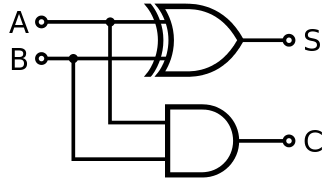
\includegraphics[scale=0.5]{halfadder}
		\caption{A half adder \autocite{rouseHalfAdder2020}.}
		\label{figure:2}
	\end{figure}
	
	While this circuit can perform addition, it has its limitations. Namely, it can only do single bit calculations. It cannot support more than one binary numbers, such tasks are possible through using full adders \autocite{HalfAdderDigital2015}. Furthermore, it can also experience some delay in computing, rendering it not ideal for fast calculations should an input be altered \autocite{HalfAdderDigital2015}.
	
	\subsubsection{Memory Circuits: Latches, Flip-flops, Counters, and Shift Registers}
	One subset of logic circuits that will be explored in this report are memory circuits. Memory circuits are defined as logic circuits that can retain information from past inputs. The most common types of these circuits are latches and flip-flops. \\
	
	Latches and flip-flops function identically the same, however there is one crucial difference between the two. Latches work by level-trigger, which indicates that it is only affected by the incoming input signals. Meanwhile, flip-flops are edge-triggered, which updates according to the input signals and also an external input signal commonly known as a "clock". Moreover, the edge-triggering mechanism can also be divided further into 2 categories, a rising edge trigger (updates when logic levels switch from low to high) and a falling edge trigger (updates when logic levels switch from high to low).
	
	Flip-flops and latches can be divided into several types: SR (Set-Reset), D (Data), and JK (it's complicated). SR and JK functions the same, if a signal is passed through the S input, it will set the output to be HIGH, and if a signal is passed through R, it will set the output to LOW ("reset"). The only difference in those two types are that SR latches disallows for both S and R to be high, while JK does allow for both to be high, functioning as a "toggle" for the output. An illustration can be found within the truth table in Table \ref{SRJKtable}.
	
	\begin{table}[h]
		\centering
		\begin{tabular}{@{}llll@{}}
			\toprule
			$S$(et) & $R$(eset) & $Q$(output) & $\overline{Q}$(negated output) \\ \midrule
			0     & 0       & No Change & No Change            \\
			1     & 0       & 1         & 0                    \\
			0     & 1       & 0         & 1                    \\
			1     & 1       & INVALID   & INVALID              \\ \bottomrule
		\end{tabular} \quad
		\begin{tabular}{@{}llll@{}}
			\toprule
			$J$(set) & $K$(reset) & $Q$(output) & $\overline{Q}$(negated output) \\ \midrule
			0     & 0       & No Change & No Change            \\
			1     & 0       & 1         & 0                    \\
			0     & 1       & 0         & 1                    \\
			1     & 1       & Toggles   & Toggles              \\ \bottomrule
		\end{tabular}
		\caption{Truth table for SR (top) and JK (bottom) types}
		\label{SRJKtable}
	\end{table}
	
	D types are an extension of the SR and JK types, as it toggles the output whenever it is inputted. Common latches and flip-flops circuit diagrams are shown in Table \ref{table:2}. \\
	\begin{table}[h]
		\centering
		\begin{tabular}{@{}lll@{}}
			\toprule
			Memory Circuit & Implementation & Circuit Symbol \\ \midrule
			SR Latch       & 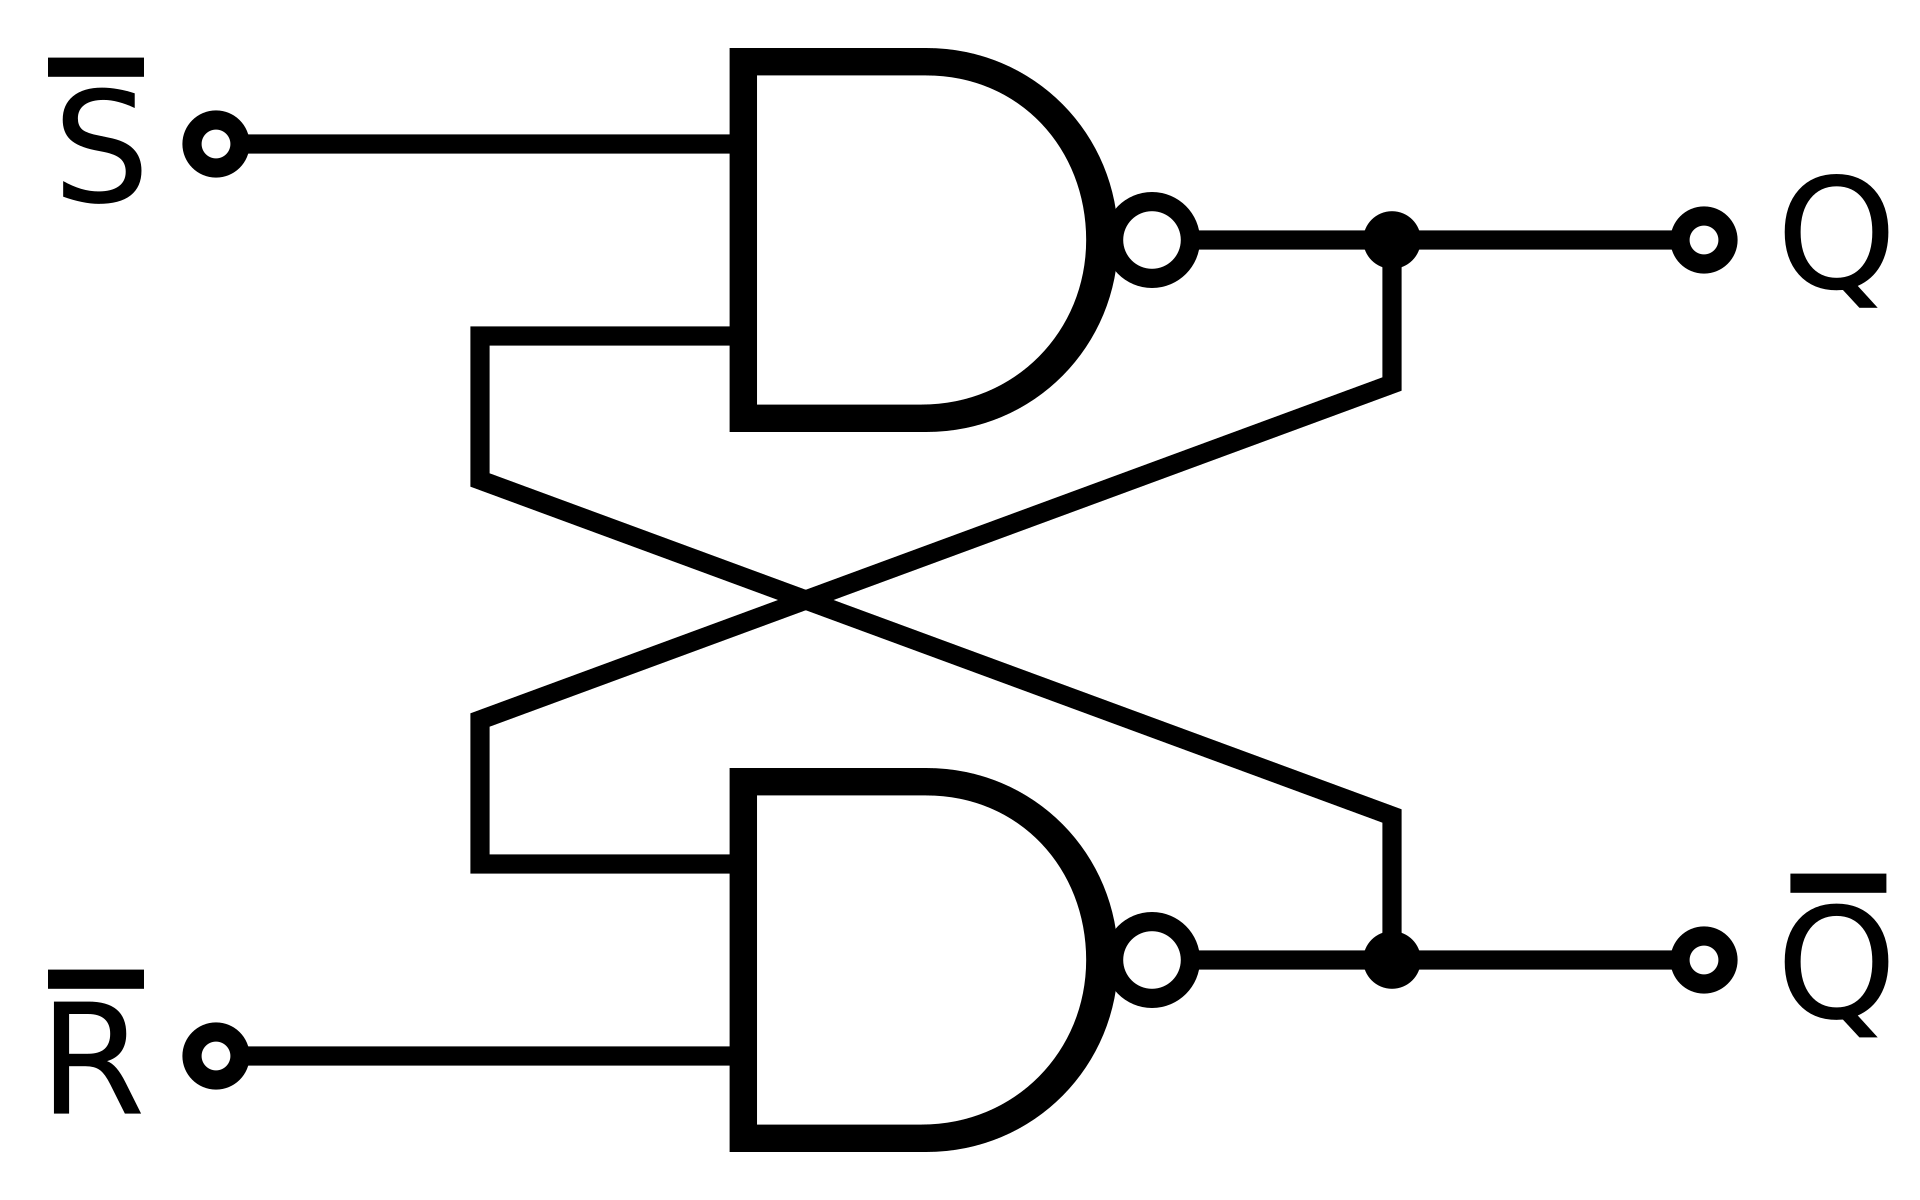
\includegraphics[scale=0.05,valign=M]{SRLatch}               & 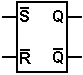
\includegraphics[scale=0.75, valign=M]{SRLatchSymbol}               \\
			JK Flip-flop   & 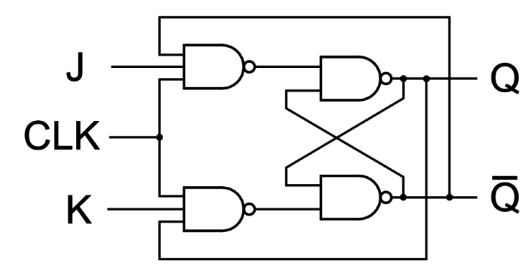
\includegraphics[scale=0.25,valign=M]{JKFlipFlop}               & 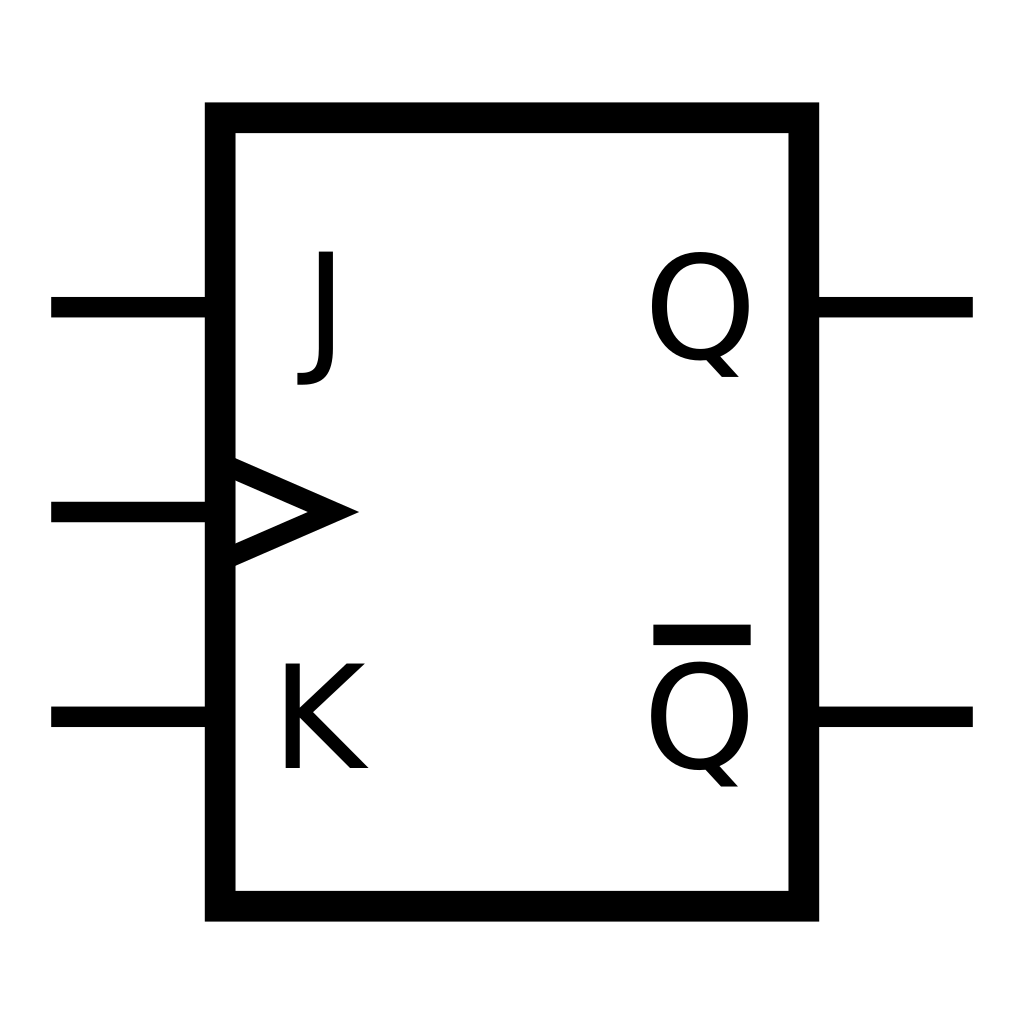
\includegraphics[scale=0.08,valign=M]{JKFlipFlopSymbol}               \\
			D Flip-flop    & 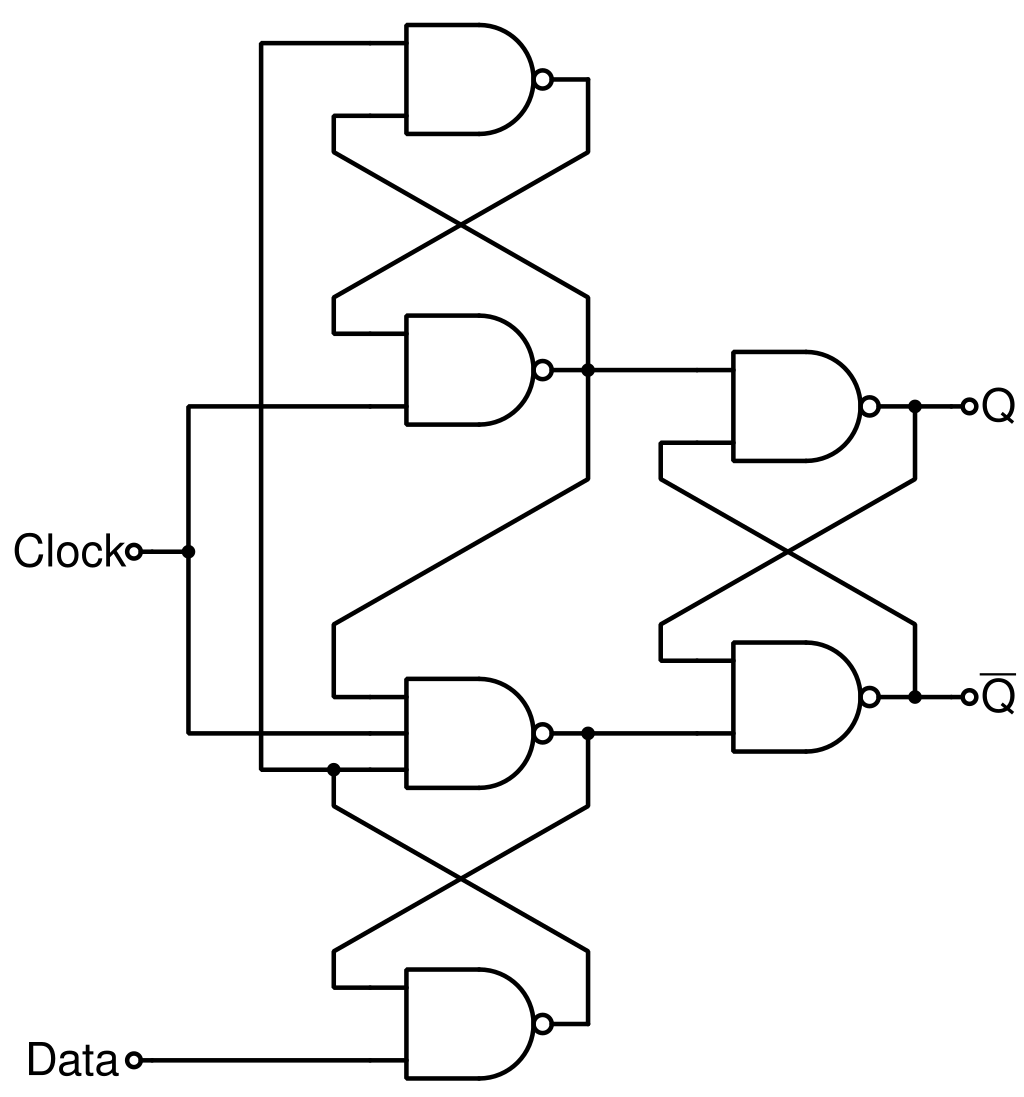
\includegraphics[scale=0.1,valign=M]{DFlipFlop}               & 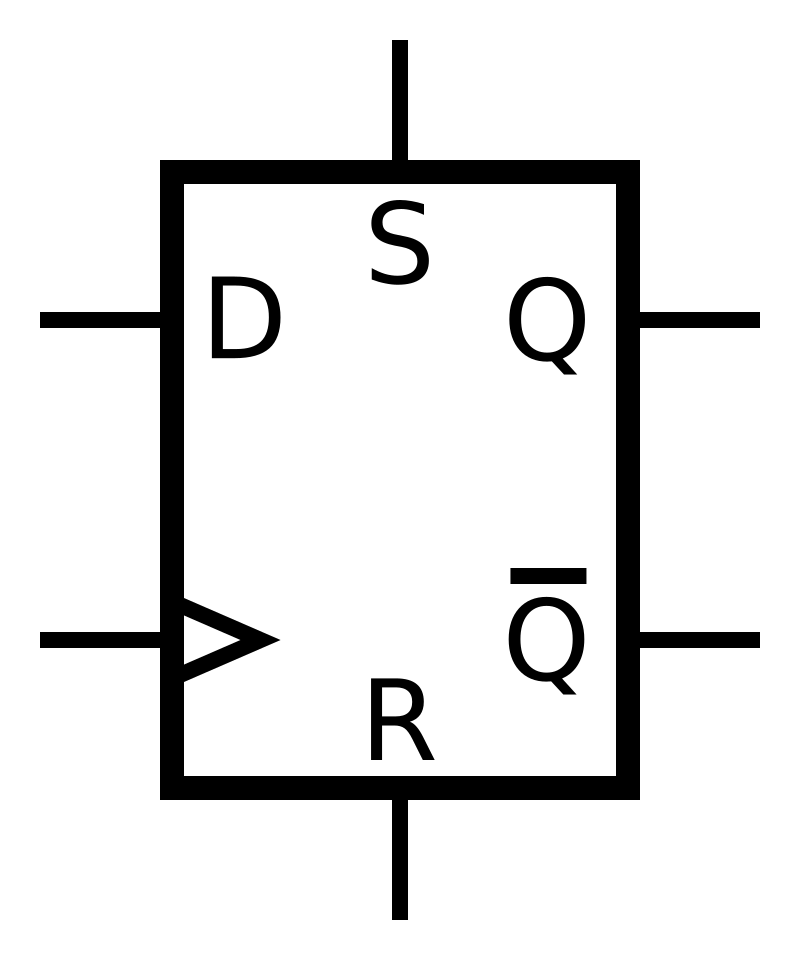
\includegraphics[scale=0.1,valign=M]{DFlipFlopSymbol}               \\ \bottomrule
		\end{tabular}
		\caption{Common memory circuit components, with their implementations and symbols \autocite{dheerajFlipFlopExplained2020,FlipflopElectronics2024}}
		\label{table:2}
	\end{table}
	
	An application for flip-flops are counters, which are practically chained flip-flops, designed to count by increments of one in binary. Counters can be subdivided into 2 categories, asynchronous and synchronous. Asynchronous counters (or ripple counters \autocite{widmerDigitalSystemsPrinciples2018}) are clocked in sequence of each flip-flops, meaning that for the next flip-flop to toggle, it needs to wait for the previous flip-flop. This is the one drawback of asynchronous counters, known as the propogation delay \autocite{widmerDigitalSystemsPrinciples2018}. However, this can be solved with the second category of counters, synchronous counters. Synchronous counters (or parallel counters \autocite{widmerDigitalSystemsPrinciples2018}) work using the same clock, as opposed to preceding flip-flop output. This leads to much faster counting which lets us handle more complicated tasks without being limited by delays \autocite{widmerDigitalSystemsPrinciples2018}. Figure \ref{figure:3} and Figure \ref{figure:4} shows the implementation of these counters. \\
	
	\begin{figure}[h]
		\centering
		\begin{minipage}{0.45\textwidth}
			\centering
			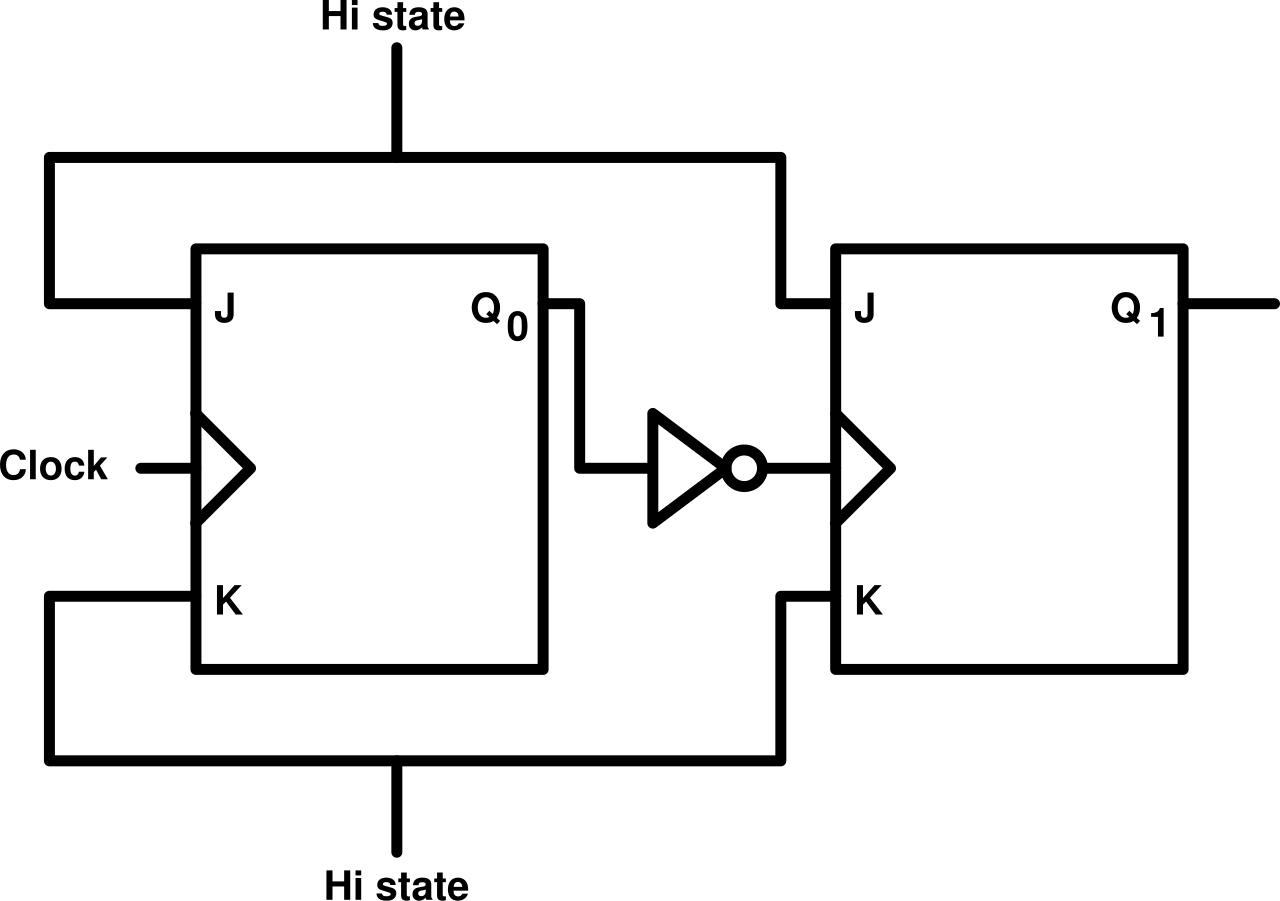
\includegraphics[scale=0.1]{asynchronous}
			\caption{A 2-bit asynchronous counter.}
			\label{figure:3}
		\end{minipage}
		\begin{minipage}{0.45\textwidth}
			\centering
			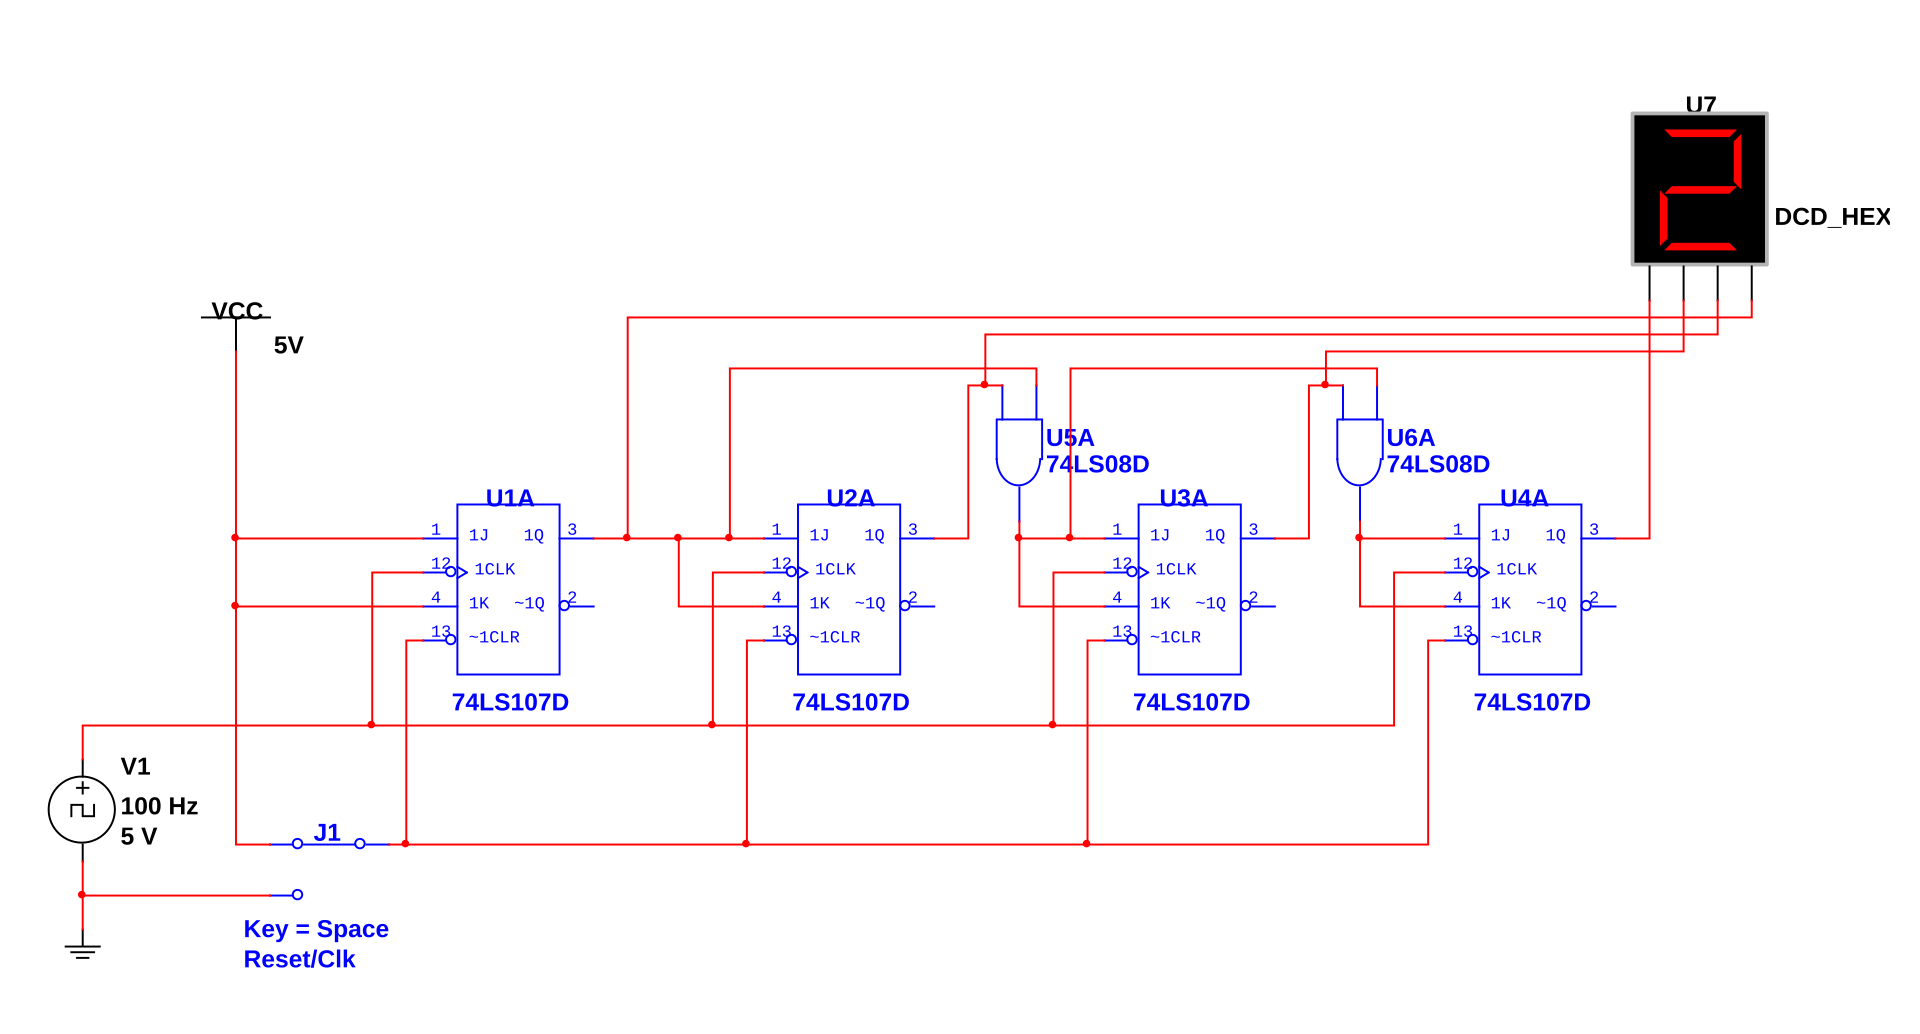
\includegraphics[scale=0.1]{synchronous}
			\caption{A 4-bit synchronous counter.}
			\label{figure:4}
		\end{minipage}
	\end{figure}
	
	However, this does not imply that the asynchronous counter is useless. In fact, the asynchronous counter could be used not as a counter, but as storage instead. This is known as the shift register. Shift registers are used for a lot of purposes, namely to convert data in series to parallel and hardware multiplication or division by 2 \autocite{xuEEE104DigitalCircuits}.
	
	For this laboratory report, we will focus on a type of shift register called a ring counter. It is named so due to the last flip-flop output of the register is connected back to the first flip-flop, hence the "ring". This also implies that so long as there is a clock pulse, the cycle keeps repeating indefinitely \autocite{widmerDigitalSystemsPrinciples2018}. \\
	
	Ring counters can also be subdivided into 2 types, the straight ring counter or the twisted ring counter \autocite{widmerDigitalSystemsPrinciples2018}. Straight ring counters, also known as one-hot counter, are ring counters that passes its state onto the next flip-flop and resets itself, and is what specialists typically refer to when describing a ring counter. Twisted ring counters, also known as Johnson counters, are ring counters that doesn't start resetting itself until the last flip-flop is active. Circuit diagrams for both types are shown in Figure \ref{figure:5} and \ref{figure:6}. 
	
	\begin{figure}[h]
		\centering
		\begin{minipage}{0.45\textwidth}
			\centering
			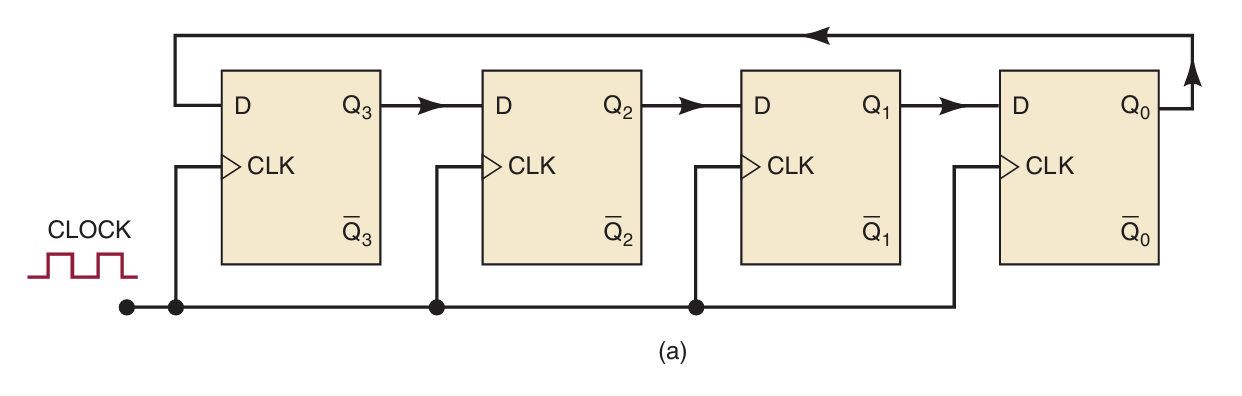
\includegraphics[scale=0.15]{Straight}
			\caption{A 4-bit straight ring counter \autocite{widmerDigitalSystemsPrinciples2018}.}
			\label{figure:5}
		\end{minipage}
		\begin{minipage}{0.45\textwidth}
			\centering
			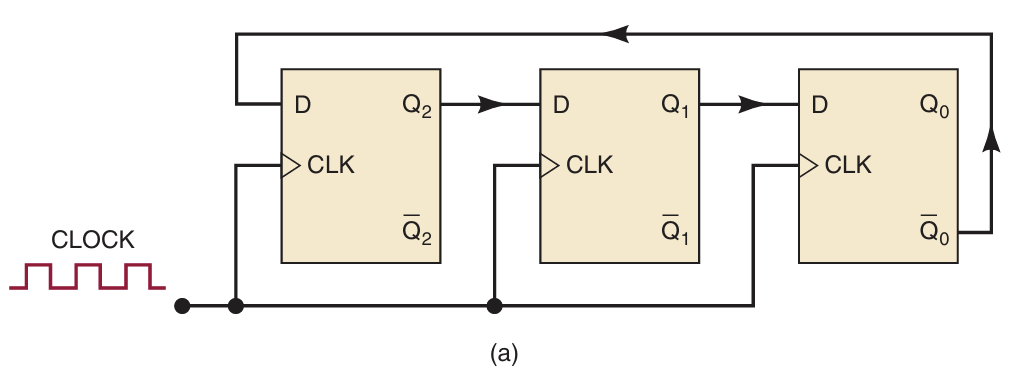
\includegraphics[scale=0.15]{Twisted}
			\caption{A 3-bit twisted ring counter \autocite{widmerDigitalSystemsPrinciples2018}.}
			\label{figure:6}
		\end{minipage}
	\end{figure}

\section{Methodology}
	The laboratory session utilized the following apparatus to conduct the experiment;
	\begin{outline}[enumerate]
		\1 NI Elvis III prototyping board and a computer running Windows 10, integrating power supplies, a function generator, and a multimetre.
		\1 Hook-up wires and 7400-series Low-power Schottky integrated circuits listed below. Definitions for the integrated circuits can be found in Appendix A.
			\2 $1$ x 74LS00 (NAND Gate)
			\2 $1$ x 74LS02 (NOR Gate)
			\2 $1$ x 74LS04 (NOT Gate)
			\2 $1$ x 74LS08 (AND Gate)
			\2 $1$ x 74LS32 (OR Gate)
			\2 $1$ x 74LS86 (XOR Gate)
			\2 $2$ x 74LS74 (D Flip-flop)
			\2 $2$ x 74LS112 (JK Flip-flop)
			\2 $4$ x $330\Omega$ Resistor
			\2 $4$ x Light-emitting diode (LED) Lights
	\end{outline}
	
	The experiment will be divided into 8 sections, and for each section, the experiment will utilize the NI Elvis III breadboard to connect the wires and logic gates. The gates will be supplied a $+5 V$ voltage signaling HIGH and the ground voltage ($0 V$) signaling LOW.
	\begin{enumerate}
		\item \textbf{Test of Basic Logic Gates}
		
		This section will examine voltage values between the output from 3 different types of logic gates (NOT gate, AND gate, and NOR gate) and the ground connection. Furthermore, the voltage values obtained will be generalized to a logic level and a truth table for each logic gate will be derived.
		
		\item \textbf{DeMorgan's Theorem}
		
		This section will prove DeMorgan's theorem by connecting 2 circuits shown in Figure \ref{demorg} and showing that their corresponding voltage values, and by extension, logic levels are equivalent. This will be proven through a truth table with all possible combinations of input.
		\begin{figure}[h]
			\centering
			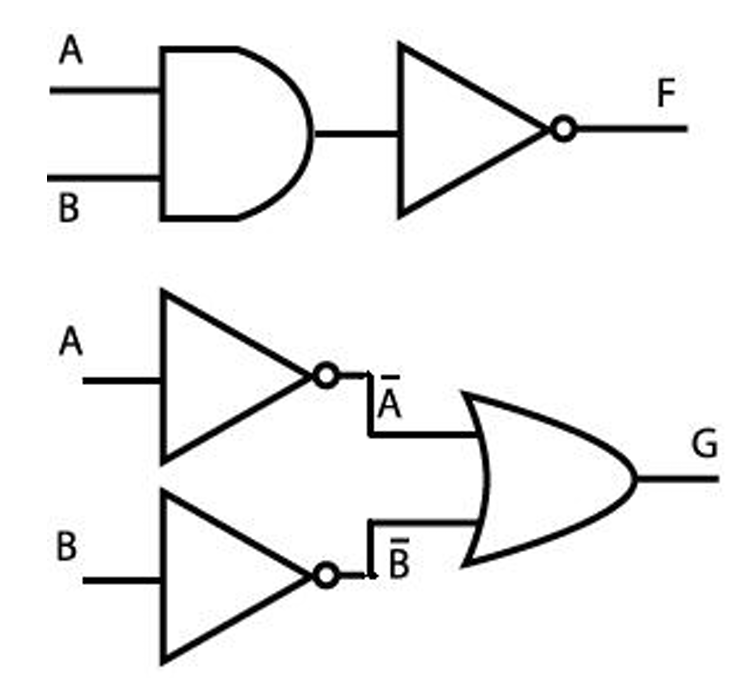
\includegraphics[scale=0.2]{demorg}
			\caption{Two circuits to prove DeMorgan's Theorem \autocite{EEE104DigitalElectronics2024}.}
			\label{demorg}
		\end{figure}
		
		\item \textbf{Combinational Logic Circuits}
		
		This section will implement a circuit based on the boolean expression $F = (A+B)(C+D)$ and a truth table will be derived based on the output signal.
		
		\item \textbf{Implementation of a Half Adder}
		
		This section will implement the half-adder circuit shown in Figure \ref{figure:2}, experimenting with its inputs, and report the output values in a truth table.
		
		\item \textbf{The S-R Latch}
		
		This section will implement the NOR version of the SR latch, shown in Figure \ref{SRNOR}. Afterwards, the circuit will be tested for all kinds of configurations, which will be documented in a truth table.
		\begin{figure}[h]
			\centering
			\begin{circuitikz} \draw 
				(0, 0) node[nor port](NOR1){}
				(0, 2) node[nor port](NOR2){}
				
				(NOR2.in 1) -- node[short]{} ++(-1, 0) -- node[above]{S} node[ocirc]{} ++(0, 0)
				(NOR1.in 2) -- node[short]{} ++(-1, 0) -- node[above]{R} node[ocirc]{} ++(0, 0)
				
				(NOR2.out) -- node[short]{} ++(1, 0) -- node[above]{$Q$} node[ocirc]{} ++(0, 0)
				(NOR1.out) -- node[short]{} ++(1, 0) -- node[above]{$\overline{Q}$} node[ocirc]{} ++(0, 0)
				
				(NOR1.out) -- ++(0,0.5) -- ($(NOR2.in 2) + (0,-0.5)$) -- (NOR2.in 2)
				(NOR2.out) -- ++(0,-0.5) -- ($(NOR1.in 1) + (0,0.5)$) -- (NOR1.in 1)
				(NOR1.out);
			\end{circuitikz}
			\caption{A NOR version of the SR latch \autocite{EEE104DigitalElectronics2024}.}
			\label{SRNOR}
		\end{figure}
		
		\item \textbf{The Edge-Triggered D Flip-flop}
		
		This section will implement the D Flip-flop shown in Figure \ref{DFF}. The truth table will be inferred and documented from this circuit.
		\begin{figure}[h]
			\centering
			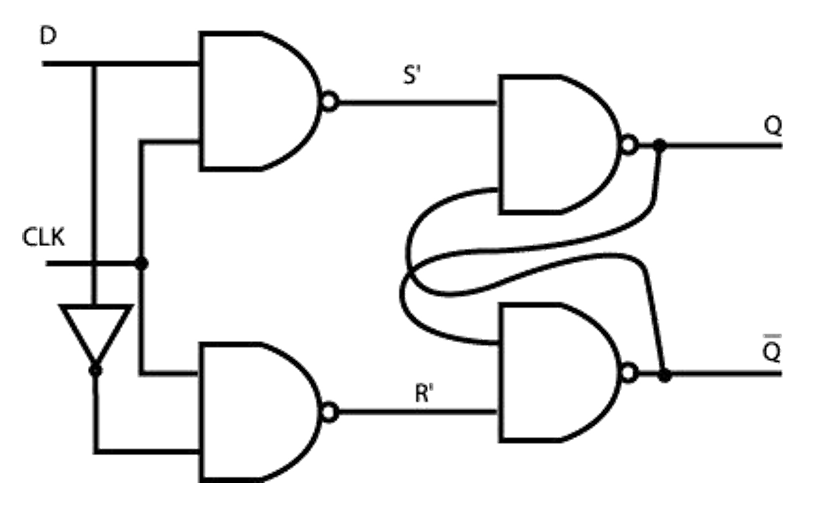
\includegraphics[scale=0.3]{DFF}
			\caption{An edge-triggered D Flip-flop \autocite{EEE104DigitalElectronics2024}.}
			\label{DFF}
		\end{figure}
		
		\item \textbf{The Asynchronous Counter}
		
		This section will implement the asynchronous counter displayed in Figure \ref{asyncCounter}. Then the flip-flops will all be reset and a clock pulse of $1~2$ Hz on the function generated will be applied to the circuit. The corresponding output will be observed in a truth table.
		\begin{figure}[h]
			\centering
			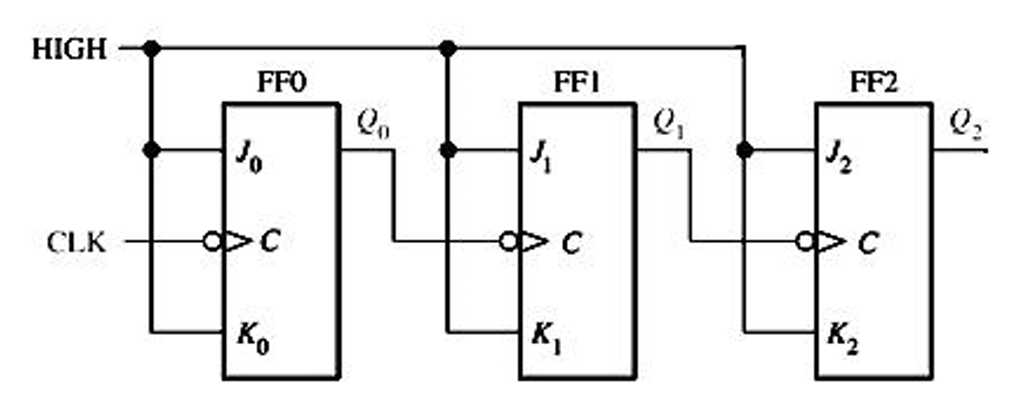
\includegraphics[scale=0.3]{asyncCount}
			\caption{An asynchronous counter \autocite{EEE104DigitalElectronics2024}.}
			\label{asyncCounter}
		\end{figure}
		
		\item \textbf{The Shift Register}
		
		This section will implement the Johnson shift register shown in Figure \ref{johnson}. A clock pulse will be registered to the circuit, similar to the previous section, and its resulting signal will be detailed in a truth table.
		\begin{figure}[h]
			\centering
			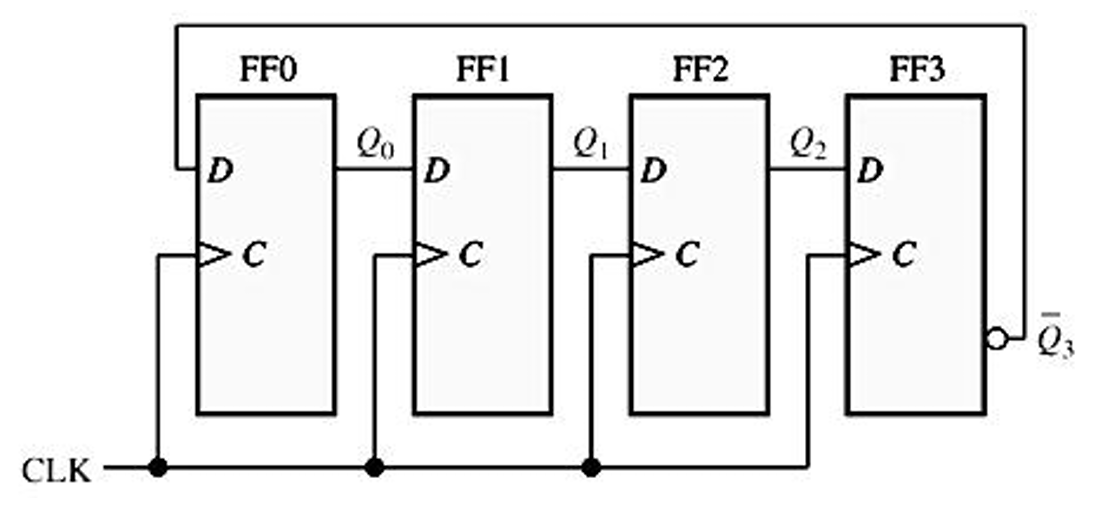
\includegraphics[scale=0.3]{johnson}
			\caption{A Johnson shift register \autocite{EEE104DigitalElectronics2024}.}
			\label{johnson}
		\end{figure}
	\end{enumerate}

\newpage
\section{Results}
	\subsection{Test of Basic Logic Gates}
	Table \ref{section1} shows the truth table for all 3 gates, both for expected values and experimental values.
	\begin{table}[h]
		\centering
		\begin{tabular}{@{}cc|cc|cc|cc@{}}
			\toprule
			\multicolumn{2}{c|}{Input} & \multicolumn{2}{c|}{NOT Gate (Input A)}                                                           & \multicolumn{2}{c|}{AND Gate} & \multicolumn{2}{c}{NOR Gate} \\ \midrule
			A            & B           & Expected                                        & Actual                                          & Expected      & Actual        & Expected     & Actual        \\ \midrule
			0 V          & 0 V         & +5 V                                            & +4.4257 V                                       & 0 V           & +0.0005 V     & +5 V         & +4.4317 V     \\
			+5 V         & 0 V         & 0 V                                             & +0.1603 V                                       & 0 V           & +0.0005 V     & 0 V          & +0.0003 V     \\
			0 V          & +5 V        & \cellcolor[HTML]{000000}{\color[HTML]{000000} } & \cellcolor[HTML]{000000}{\color[HTML]{000000} } & 0 V           & +0.0005 V     & 0 V          & +0.0003 V     \\
			+5 V         & +5 V        & \cellcolor[HTML]{000000}{\color[HTML]{000000} } & \cellcolor[HTML]{000000}{\color[HTML]{000000} } & +5 V          & +4.9965 V     & 0 V          & +0.0001 V     \\ \bottomrule
		\end{tabular}
		\caption{Truth Table for NOT, AND, and NOR gate.}
		\label{section1}
	\end{table}

	\subsection{DeMorgan's Theorem}
	Table \ref{section2} shows the truth table for both gates, as well as their expected values.
	\begin{table}[h]
		\centering
		\begin{tabular}{@{}cc|cc|cc@{}}
			\toprule
			\multicolumn{2}{c|}{Inputs} & \multicolumn{2}{c|}{NAND Gate} & \multicolumn{2}{c}{Negative OR Gate} \\ \midrule
			A            & B            & Expected      & Actual         & Expected         & Actual            \\ \midrule
			0 V          & 0 V          & +5 V          & +4.4324 V      & +5 V             & +4.9944 V         \\
			+5 V         & 0 V          & +5 V          & +4.4335 V      & +5 V             & +4.9938 V         \\
			0 V          & +5 V         & +5 V          & +4.4335 V      & +5 V             & +4.9938 V         \\
			+5 V         & +5 V         & 0 V           & +0.0003 V      & 0 V              & +0.0009 V         \\ \bottomrule
		\end{tabular}
		\caption{Truth Table to prove DeMorgan's Theorem.}
		\label{section2}
	\end{table}
	
	\newpage
	\subsection{Combinational Logic Circuits}
	Table \ref{section3} shows the truth table for the given Boolean expression, $F = (A+B)(C+D)$.
	\begin{table}[h]
		\centering
		\begin{tabular}{@{}cccc|cc@{}}
			\toprule
			\multicolumn{4}{c|}{Inputs} & \multicolumn{2}{c}{Output (F)} \\ \midrule
			A     & B     & C    & D    & Expected      & Actual         \\ \midrule
			0 V   & 0 V   & 0 V  & 0 V  & 0 V           & +0.0001 V      \\
			+5 V  & 0 V   & 0 V  & 0 V  & 0 V           & +0.0005 V      \\
			0 V   & +5 V  & 0 V  & 0 V  & 0 V           & +0.0005 V      \\
			+5 V  & +5 V  & 0 V  & 0 V  & 0 V           & +0.0003 V      \\
			0 V   & 0 V   & +5 V & 0 V  & 0 V           & +0.0005 V      \\
			+5 V  & 0 V   & +5 V & 0 V  & +5 V          & +4.9986 V      \\
			0 V   & +5 V  & +5 V & 0 V  & +5 V          & +4.9986 V      \\
			+5 V  & +5 V  & +5 V & 0 V  & +5 V          & +4.9941 V      \\
			0 V   & 0 V   & 0 V  & +5 V & 0 V           & +0.0005 V      \\
			+5 V  & 0 V   & 0 V  & +5 V & +5 V          & +4.9986 V      \\
			0 V   & +5 V  & 0 V  & +5 V & +5 V          & +4.9986 V      \\
			+5 V  & +5 V  & 0 V  & +5 V & +5 V          & +4.9941 V      \\
			0 V   & 0 V   & +5 V & +5 V & 0 V           & +0.0003 V      \\
			+5 V  & 0 V   & +5 V & +5 V & +5 V          & +4.9941 V      \\
			0 V   & +5 V  & +5 V & +5 V & +5 V          & +4.9941 V      \\
			+5 V  & +5 V  & +5 V & +5 V & +5V           & +4.9937 V      \\ \bottomrule
		\end{tabular}
		\caption{Truth table for the boolean expression in Section 3.}
		\label{section3}
	\end{table}
	
	\subsection{Implementation of a Half-adder}
	Table \ref{section4} shows the truth table of the implemented half-adder.
	\begin{table}[h]
		\centering
		\begin{tabular}{@{}cc|cccc@{}}
			\toprule
			\multicolumn{2}{c|}{Inputs}                         & \multicolumn{4}{c}{Outputs}                                           \\ \midrule
			\cellcolor[HTML]{000000} & \cellcolor[HTML]{000000} & \multicolumn{2}{c|}{Expected}            & \multicolumn{2}{c}{Actual} \\ \midrule
			A                        & B                        & XOR Gate & \multicolumn{1}{c|}{AND Gate} & XOR Gate     & AND Gate    \\ \midrule
			0 V                      & 0 V                      & 0 V      & \multicolumn{1}{c|}{0 V}      & +0.1584 V    & -0.0008 V   \\
			+5 V                     & 0 V                      & +5 V     & \multicolumn{1}{c|}{0 V}      & +4.4175 V    & +0.0006 V   \\
			0 V                      & +5 V                     & +5 V     & \multicolumn{1}{c|}{0 V}      & +4.4175 V    & +0.0006 V   \\
			+5 V                     & +5 V                     & 0 V      & \multicolumn{1}{c|}{+5 V}     & +0.1681 V    & +4.9874 V   \\ \bottomrule
		\end{tabular}
		\caption{Truth table for a half-adder.}
		\label{section4}
	\end{table}
	
	\subsection{The SR Latch}
	Table \ref{section5} shows the truth table of an SR Latch, complete with previous states of the circuit.
	\begin{table}[h]
		\centering
		\begin{tabular}{@{}cc|cc|cccc@{}}
			\toprule
			\multicolumn{2}{c|}{Previous State}                 & \multicolumn{2}{c|}{Inputs}                         & \multicolumn{4}{c}{Output}                                                     \\ \midrule
			\cellcolor[HTML]{000000} & \cellcolor[HTML]{000000} & \cellcolor[HTML]{000000} & \cellcolor[HTML]{000000} & \multicolumn{2}{c|}{Expected}                    & \multicolumn{2}{c}{Actual}  \\ \midrule
			$Q_{n}$                        & $\overline{Q_{n}}$                    & S                        & R                        & $Q_{n+1}$ & \multicolumn{1}{c|}{$\overline{Q_{n+1}}$} & $Q_{n+1}$ & $\overline{Q_{n+1}}$ \\ \midrule
			0                        & 1                        & 0                        & 0                        & 0          & \multicolumn{1}{c|}{1}              & 0          & 1              \\
			1                        & 0                        & 0                        & 0                        & 1          & \multicolumn{1}{c|}{0}              & 1          & 0              \\
			0                        & 1                        & 0                        & 1                        & 0          & \multicolumn{1}{c|}{1}              & 0          & 1              \\
			1                        & 0                        & 0                        & 1                        & 0          & \multicolumn{1}{c|}{1}              & 0          & 1              \\
			0                        & 1                        & 1                        & 0                        & 1          & \multicolumn{1}{c|}{0}              & 1          & 0              \\
			1                        & 0                        & 1                        & 0                        & 1          & \multicolumn{1}{c|}{0}              & 1          & 0              \\
			0                        & 1                        & 1                        & 1                        & Random     & \multicolumn{1}{c|}{Random}         & 0          & 0              \\
			1                        & 0                        & 1                        & 1                        & Random     & \multicolumn{1}{c|}{Random}         & 0          & 0              \\ \bottomrule
		\end{tabular}
		\caption{Truth table for the SR Latch.}
		\label{section5}
	\end{table}
	
	\subsection{The Edge-triggered D Flip-flop}
	Table \ref{section6} shows the truth table of an edge-triggered D flip-flop, along with the previous states of the circuit.
	\begin{table}[h]
		\centering
		\begin{tabular}{@{}cc|c|cccc@{}}
			\toprule
			\multicolumn{2}{c|}{Previous State}                 & Input                    & \multicolumn{4}{c}{Output}                                 \\ \midrule
			\cellcolor[HTML]{000000} & \cellcolor[HTML]{000000} & \cellcolor[HTML]{000000} & \multicolumn{2}{c|}{Expected} & \multicolumn{2}{c}{Actual} \\ \midrule
			$Q_{n}$                        & $\overline{Q_{n}}$                     & D                        & $Q_{n+1}$  & \multicolumn{1}{c|}{$\overline{Q_{n+1}}$} & $Q_{n+1}$           & $\overline{Q_{n+1}}$          \\ \midrule
			0                        & 1                        & 0                        & 0   & \multicolumn{1}{c|}{1}  & 0            & 1           \\
			1                        & 0                        & 0                        & 1   & \multicolumn{1}{c|}{0}  & 1            & 0           \\
			0                        & 1                        & 1                        & 1   & \multicolumn{1}{c|}{0}  & 1            & 0           \\
			1                        & 0                        & 1                        & 0   & \multicolumn{1}{c|}{1}  & 0            & 1           \\ \bottomrule
		\end{tabular}
		\caption{Truth table for an edge-triggered D flip-flop.}
		\label{section6}
	\end{table}
	
	\subsection{The Asynchronous Counter}
	Table \ref{section7} shows the sequence table of the three output values of the flip-flops.
	\begin{table}[h]
		\centering
		\begin{tabular}{@{}c|cccccc@{}}
			\toprule
			\cellcolor[HTML]{000000} & \multicolumn{6}{c}{Circuit State}                                              \\ \midrule
			\cellcolor[HTML]{000000} & \multicolumn{3}{c|}{Expected}                    & \multicolumn{3}{c}{Actual}  \\ \midrule
			Clock Cycle              & $Q_{0}$ & $Q_{1}$ & \multicolumn{1}{c|}{$Q_{2}$} & $Q_{0}$ & $Q_{1}$ & $Q_{2}$ \\ \midrule
			Initial                  & 0       & 0       & \multicolumn{1}{c|}{0}       & 0       & 0       & 0       \\
			1                        & 1       & 0       & \multicolumn{1}{c|}{0}       & 1       & 0       & 0       \\
			2                        & 0       & 1       & \multicolumn{1}{c|}{0}       & 0       & 1       & 0       \\
			3                        & 1       & 1       & \multicolumn{1}{c|}{0}       & 1       & 1       & 0       \\
			4                        & 0       & 0       & \multicolumn{1}{c|}{1}       & 0       & 0       & 1       \\
			5                        & 1       & 0       & \multicolumn{1}{c|}{1}       & 1       & 0       & 1       \\
			6                        & 0       & 1       & \multicolumn{1}{c|}{1}       & 0       & 1       & 1       \\
			7                        & 1       & 1       & \multicolumn{1}{c|}{1}       & 1       & 1       & 1       \\
			8                        & 0       & 0       & \multicolumn{1}{c|}{0}       & 0       & 0       & 0       \\
			9                        & 1       & 0       & \multicolumn{1}{c|}{0}       & 1       & 0       & 0       \\ \bottomrule
		\end{tabular}
		\caption{Sequence table for an asynchronous counter.}
		\label{section7}
	\end{table}
	
	Note that the 8th and 9th tick are equal to the initial and 1st tick. This suggests that the counter is in an indefinite cycle.
	
	\subsection{The Shift Register}
	Table \ref{section8} shows the sequence table of the Johnson Register at each clock step.
	\begin{table}[h]
		\centering
		\begin{tabular}{@{}c|ccclcccl@{}}
			\toprule
			\cellcolor[HTML]{000000}                        & \multicolumn{8}{c}{Circuit State}                                   \\ \midrule
			\cellcolor[HTML]{000000}{\color[HTML]{000000} } & \multicolumn{4}{c|}{Expected}          & \multicolumn{4}{c}{Actual} \\ \midrule
			Clock Cycle                                     & $Q_{0}$ & $Q_{1}$ & $Q_{2}$ & \multicolumn{1}{l|}{$Q_{3}$} & $Q_{0}$    & $Q_{1}$   & $Q_{2}$   & $Q_{3}$   \\ \midrule
			Initial                                         & 0  & 0  & 0  & \multicolumn{1}{l|}{0}  & 0  & 0  & 0  & 0                     \\
			1                                               & 1  & 0  & 0  & \multicolumn{1}{c|}{0}  & 1  & 0  & 0  & \multicolumn{1}{c}{0} \\
			2                                               & 1  & 1  & 0  & \multicolumn{1}{c|}{0}  & 1  & 1  & 0  & \multicolumn{1}{c}{0} \\
			3                                               & 1  & 1  & 1  & \multicolumn{1}{c|}{0}  & 1  & 1  & 1  & \multicolumn{1}{c}{0} \\
			4                                               & 1  & 1  & 1  & \multicolumn{1}{l|}{1}  & 1  & 1  & 1  & 1                     \\
			5                                               & 0  & 1  & 1  & \multicolumn{1}{l|}{1}  & 0  & 1  & 1  & 1                     \\
			6                                               & 0  & 0  & 1  & \multicolumn{1}{l|}{1}  & 0  & 0  & 1  & 1                     \\
			7                                               & 0  & 0  & 0  & \multicolumn{1}{l|}{1}  & 0  & 0  & 0  & 1                     \\
			8                                               & 0  & 0  & 0  & \multicolumn{1}{l|}{0}  & 0  & 0  & 0  & 0                     \\ \bottomrule
		\end{tabular}
		\caption{Sequence table for a Johnson shift register.}
		\label{section8}
	\end{table}
	
	Notice that this shares a similarity with the previous section, that is, it loops indefinitely.
	
\section{Discussion}
	This section will be split into 2 sections, one for the general result gathered from the experiment and comparing it to the expected theoretical results, and another one for further discussions on selected sections, as required by the laboratory regulations.

	\subsection{General Result Discussion}
		The results from the preceding section matched what the expected output is. However, there are still discrepancy between the two values. Namely, the voltage output is not exact. This might be caused by the resistors residing in the integrated chip used for this laboratory. The expected voltages are ideal, meaning that an assumption was made to have "perfect resistors", meaning that the wires inside the logic chip had no resistance. However, the real world is far from ideal, therefore small errors like it exists.

		Furthermore, there are more glaring value discrepancies found in the result of some sections of the experiment. This might be due to the fact that the measurement of the voltage was not perfect, or the implementation of the chip was crooked. This can cause a larger voltage difference from the actual voltage. However, this does not pose a problem for this experiment, as readings could still be inferred as HIGH or LOW for a suitable range.

		The only incorrect hypothesis was found in the SR latch section. The original hypothesis was that if both S and R were HIGH, then the expected output would be random, hence why the need to ban such inputs. However, this hypothesis was not correct. What the circuit actually does is that when both are set to HIGH, both resulting outputs are set to LOW \autocite{neil_ukAnswerWhatActually2017}. The reason behind why this is not allowed is when both S and R return back to LOW \autocite{neil_ukAnswerWhatActually2017}. In which case, propogation delay will decide which switch would turn on, which for the human observer, would essentially be randomized \autocite{neil_ukAnswerWhatActually2017}. 

	\subsection{Particular Sections Discussion}
		In section 2, we have proven the DeMorgan's Theorem by physically implementing the equivalent circuits and examined the output for both circuits. To prove that its boolean expression are equivalent, it can be showed that the first circuit has the boolean expression $\overline{AB}$, while the second circuit has the expression $\overline{A} + \overline{B}$. Since it has been proven that the first and second circuit are equivalent by the truth table in Table \ref{section2}, we can conclude that $\overline{AB} = \overline{A} + \overline{B}$, as required. \\
		
		In section 4, our experimental results matched our expected results, meaning arithmetic is possible with this circuit. However, as discussion in the Preliminary Information section, half-adders are not sufficient to implement basic binary arithmetic, as it can only handle single bit addition, not sufficient for carry calculations. Most complex digital circuits almost always needs a binary calculator that can handle more than one bit and the possibility of chaining carry bits (i.e. 0111 to 1000). \\
		
		In section 5, we implemented the SR latch and observed its inputs based on previous states and the S and R input. However, to explain in further detail on why the circuit behaves like expected, it is important to understand the step-by-step process behind it.
		
		Regardless of if the circuit has been initialized or not, the output for an SR latch is forcibly decided on if either S or R is set to HIGH. In the case that S and R are both set to HIGH, then both outputs will return LOW. This is what was observed in the results section above, and more details regarding both S and R being HIGH were explained in the previous subsection.
		
		However, the more interesting behavior of this circuit is when both S and R are low. If the circuit is initialized in this configuration, at least one of the output will be HIGH. This decision is made purely at random based on speed and propogation delay, as discussed previously. Then, once either one is set to HIGH, if both inputs are LOW then it will stay at that state, which is what the intersection wires in the middle are for. The circuit "remembers" the state, thus, it is a memory circuit. \\
		
		In section 6, the experiment investigated the D flip-flop and its output based on the D input and the previous states. Much like the preceding section related to the SR latch, we will also try and explain how the D flip-flop works.
		
		The D flip-flop is essentially an extension of the SR latch. However, it is complicated by the 2 NAND gates and the clock signal before it. The D signal is responsible for deciding if the output should be set to HIGH or LOW. If D is LOW, then output is set to LOW, and vice-versa. This is what is found in the truth table above. It can store this data because of the clock, as the clock is being actively blocked by the D signal in the first two NAND gates. D flip-flops have applications in shift registers, which we will discuss later in this report. \\
		
		In section 7, the experiment implemented a $3$-bit asynchronous counter and documented its results in the truth table in the results section. Generalizing the results, we can see that for an $n$-bit counter, we can count up to $2^n$. The range for this count goes from $0$ to $2^n - 1$.
		
		This circuit can count because of the cascading flip-flops utilized here. To see this generally, suppose that $k$ is an integer between $2$ and $n$. We can see that the $k$-th flip-flop cannot toggle if the $k-1$-th flip-flop doesn't provide an update in the form of the clock. Since $k$ can be any value between that range, all the flip-flops can only be updated if the first flip-flop updates periodically. Thus, counting can be achieved.
		
		There is another type of counters called the synchronous counters, which we have explained in the preliminary information section of this report. To summarize, synchronous counters don't rely on the first flip-flop to update. Instead, the same clock signal is connected to every circuit, with the output for one flip-flop connected to the following flip-flops.

\section{Conclusion}
	This report has demonstrated and verified some concepts of digital circuits that are instrumental to nearly every digital devices present. Namely, we have discussed logic gates and Boolean Algebra, as well as combinational logic circuits and memory circuits. \\
	
	While a successful laboratory experience was achieved, there are still some shortcomings that needed to be addressed for future sessions. First is regarding group work in the context of the laboratory. While a clear division of tasks was implemented, understanding of the material may not be equal amongst the laboratory participants. Thus, it is suggested that for future sessions, group members for the session are encouraged to try their hands on doing the field work, as opposed to documenting the results. 
	
	Moreover, this report was the author's third experience writing in \LaTeX, and more features and extensions of this software could be used to professionalize this report by using specialized tools to draw figures and diagrams. Software such as CircuiTikz could have been used to produce higher quality circuit figures, however a lack of experience has made it difficult and time-consuming for the author. \\
	
	This laboratory session has been enlightening and has reinforced the theoretical knowledge presented in the lectures and assignments. More opportunities for students to try and design logic circuits should stimulate their knowledge and desire to learn more about this subject.

\printbibliography

\end{document}